%!TeX root=../../tcc.tex


\chapter{Triangulação de Delaunay cinética}\label{ch:triangulacao-de-delaunay-cinetica}

% Descrever o problema cinético

Considere o seguinte problema cinético.
São dados $n$ pontos movendo-se linearmente no plano.
Cada ponto é representado por um par $(s_0, \vec{v})$ onde $s_0 = (x_0, y_0)$ é a sua posição
inicial e $\vec{v} = (v_x, v_y)$ um vetor velocidade.
A posição de um determinado ponto $p$, num instante arbitrário $t \geq 0$, é
$s_p = (x_p, y_p) = (x_0, y_0)+t\cdot \vec{v}$.
Queremos saber o conjunto de arestas que define a triangulação de Delaunay desses pontos, num
instante arbitrário $t \geq 0$.

Por exemplo, esta é a triangulação de Delaunay para os 8 pontos na coleção representada na
Figura~\ref{fig:delaunay:exemplo}:
%$((-2, -1), \left(\frac{5}{4}, \frac{1}{2}\right))$, $\left((-1, 3), \left(\frac{1}{2}, -1\right)
%\right)$, $((1, 1), (1, -1))$, $((1, 2), (1, 0))$, $((2, 0), (0, -1))$, $((2, -2), (2, -1))$,
%$((3, 4), (2,-2))$, $\left((4, 2), \left(-\frac{3}{2}, 1\right)\right)$.

\begin{figure}[H]
    \centering
    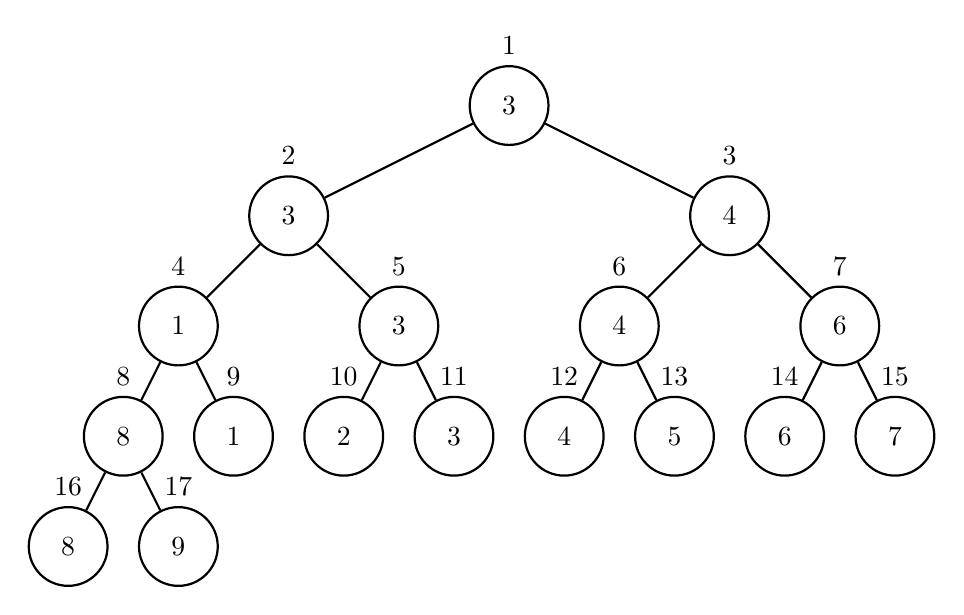
\begin{tikzpicture}[thick, scale=0.7]
        \node[label={1},circle,draw,minimum size=1cm]
        (1) at (0,0) {$3$};
        \node[label={2},circle,draw,minimum size=1cm]
        (2) at (-4,-2) {$3$};
        \node[label={3},circle,draw,minimum size=1cm]
        (3) at (4,-2) {$4$};
        \node[label={4},circle,draw,minimum size=1cm]
        (4) at (-6,-4) {$1$};
        \node[label={5},circle,draw,minimum size=1cm]
        (5) at (-2,-4) {$3$};
        \node[label={6},circle,draw,minimum size=1cm]
        (6) at (2,-4) {$4$};
        \node[label={7},circle,draw,minimum size=1cm]
        (7) at (6,-4) {$6$};
        \node[label={8},circle,draw,minimum size=1cm]
        (8) at (-7,-6) {$8$};
        \node[label={9},circle,draw,minimum size=1cm]
        (9) at (-5,-6) {$1$};
        \node[label={10},circle,draw,minimum size=1cm]
        (10) at (-3,-6) {$2$};
        \node[label={11},circle,draw,minimum size=1cm]
        (11) at (-1,-6) {$3$};
        \node[label={12},circle,draw,minimum size=1cm]
        (12) at (1,-6) {$4$};
        \node[label={13},circle,draw,minimum size=1cm]
        (13) at (3,-6) {$5$};
        \node[label={14},circle,draw,minimum size=1cm]
        (14) at (5,-6) {$6$};
        \node[label={15},circle,draw,minimum size=1cm]
        (15) at (7,-6) {$7$};
        \node[label={16},circle,draw,minimum size=1cm]
        (16) at (-8,-8) {$8$};
        \node[label={17},circle,draw,minimum size=1cm]
        (17) at (-6,-8) {$9$};

        \draw[thick] (1) -- (2);
        \draw[thick] (2) -- (4);
        \draw[thick] (4) -- (8);
        \draw[thick] (4) -- (9);
        \draw[thick] (8) -- (16);
        \draw[thick] (8) -- (17);
        \draw[thick] (2) -- (5);
        \draw[thick] (5) -- (10);
        \draw[thick] (5) -- (11);
        \draw[thick] (1) -- (3);
        \draw[thick] (3) -- (6);
        \draw[thick] (3) -- (7);
        \draw[thick] (6) -- (12);
        \draw[thick] (6) -- (13);
        \draw[thick] (7) -- (14);
        \draw[thick] (7) -- (15);
    \end{tikzpicture}
    \caption[Representação da estrutura torneio]{Torneio com $9$
        elementos em que $3$ é o elemento com valor máximo.}
    \label{fig:torneio:exemplo}
\end{figure}

Para entender o que é a triangulação de Delaunay de um conjunto de pontos, precisamos antes
entender o que é o diagrama de Voronoi.

O diagrama de Voronoi de um conjunto $P$ de pontos é uma partição do plano em regiões que
correspondem aos pontos de $p$.
Cada região $R(p)$ compreende todos os pontos do plano mais próximos de $p$ do que de qualquer
outro ponto do conjunto $P$.
As regiões são polígonos cujas arestas são formadas por pontos que estão equidistantes de dois ou
mais pontos de $P$.
Os vértices desse polígono estão equidistantes de três ou mais pontos de $P$.
Veja a Figura~\ref{fig:delaunay:voronoi}.

\begin{figure}[H]
    \centering
    \begin{tikzpicture}[scale=0.7]
        \node[label={[label distance = -3mm]160:$a$}] at (-3.0, 0) {\textbullet};
        \node[label={[label distance = -3mm]160:$b$}] at (1, 1) {\textbullet};
        \node[label={[label distance = -3mm]160:$c$}] at (3.5, 4.0) {\textbullet};
        \node[label={[label distance = -3mm]160:$d$}] at (0, 3) {\textbullet};
        \node[label={[label distance = -3mm]160:$e$}] at (1, 5) {\textbullet};
        \node[label={[label distance = -3mm]160:$f$}] at (-2.0, 4) {\textbullet};
        \node[label={[label distance = -3mm]160:$g$}] at (-4, 6) {\textbullet};

        \node (abd) at (-1.1666666666666667, 1.1666666666666667) {\textbullet}; % a-b-d
        \draw (-1.1666666666666667, 1.1666666666666667) -- (-1.8333333333333333, 1.8333333333333333); %abd--afd
        \draw (-1.1666666666666667, 1.1666666666666667) -- (1.96875, 2.734375); %abd--dbc
% a -- b
        \draw (-1.1666666666666667, 1.1666666666666667) -- (-0.6815954165940006, -0.773618333623997);
        \node (afd) at (-1.8333333333333333, 1.8333333333333333) {\textbullet}; % a-f-d
        \draw (-1.8333333333333333, 1.8333333333333333) -- (-0.5, 4.5); %afd--fed
        \draw (-1.8333333333333333, 1.8333333333333333) -- (-5.3, 2.7); %afd--afg
        \node (dbc) at (1.96875, 2.734375) {\textbullet}; % d-b-c
% b -- c
        \draw (1.96875, 2.734375) -- (3.505192559194752, 1.4540062006710404);
        \node (afg) at (-5.3, 2.7) {\textbullet}; % a-f-g
% g -- a
        \draw (-5.3, 2.7) -- (-7.272787847664287, 2.3712020253892856);
        \node (fge) at (-1.25, 6.75) {\textbullet}; % f-g-e
        \draw (-1.25, 6.75) -- (-0.5, 4.5); %fge--fed
        \draw (-1.25, 6.75) -- (-5.3, 2.7); %fge--afg
% e -- g
        \draw (-1.25, 6.75) -- (-0.8577677297236319, 8.71116135138184);
        \node (fed) at (-0.5, 4.5) {\textbullet}; % f-e-d
        \node (edc) at (1.7916666666666667, 3.3541666666666665) {\textbullet}; % e-d-c
        \draw (1.7916666666666667, 3.3541666666666665) -- (-0.5, 4.5); %edc--fed
        \draw (1.7916666666666667, 3.3541666666666665) -- (1.96875, 2.734375); %edc--dbc
% c -- e
        \draw (1.7916666666666667, 3.3541666666666665) -- (2.534448019374874, 5.211120048437185);


    \end{tikzpicture}
    \caption[Exemplo de diagrama de Voronoi]{Exemplo de diagrama de Voronoi.}\label{fig:delaunay:voronoi}
\end{figure}

A triangulação de Delaunay de um conjunto de pontos $P$ é definida como a triangulação do grafo
dual do diagrama de Voronoi para $P$.
Os vértices do grafo dual são os pontos de $P$ e para cada região associada ao ponto no diagrama de
Voronoi existe uma aresta entre o vértice associado à região e os vértices associados às regiões
adjacentes.
Veja a Figura~\ref{fig:delaunay:dual}.
O grafo dual é chamado de grafo de Delaunay e a triangulação desse grafo é chamada de triangulação
de Delaunay.

\begin{figure}[H]
    \centering
    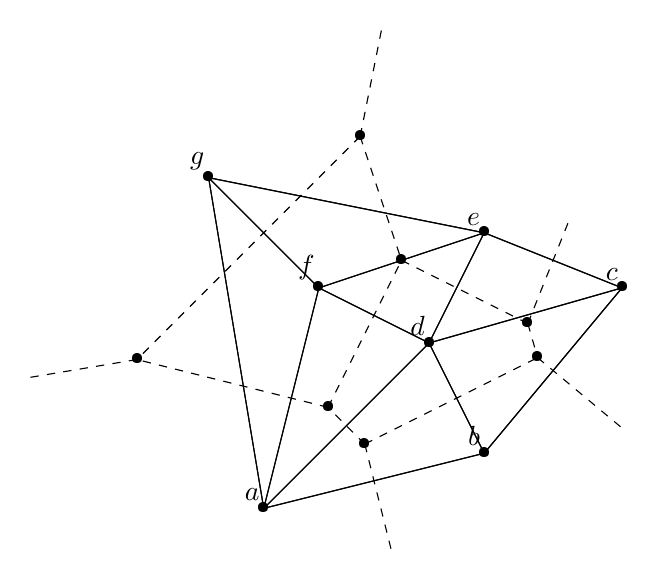
\begin{tikzpicture}[scale=0.7]
        \node[label={[label distance = -3mm]160:$a$}] at (-3.0, 0) {\textbullet};
        \node[label={[label distance = -3mm]160:$b$}] at (1, 1) {\textbullet};
        \node[label={[label distance = -3mm]160:$c$}] at (3.5, 4.0) {\textbullet};
        \node[label={[label distance = -3mm]160:$d$}] at (0, 3) {\textbullet};
        \node[label={[label distance = -3mm]160:$e$}] at (1, 5) {\textbullet};
        \node[label={[label distance = -3mm]160:$f$}] at (-2.0, 4) {\textbullet};
        \node[label={[label distance = -3mm]160:$g$}] at (-4, 6) {\textbullet};
        \draw (-3.0, 0) -- (1, 1);
        \draw (1, 1) -- (-3.0, 0);
        \draw (0, 3) -- (1, 1);
        \draw (1, 1) -- (0, 3);
        \draw (3.5, 4.0) -- (1, 1);
        \draw (1, 1) -- (3.5, 4.0);
        \draw (-3.0, 0) -- (0, 3);
        \draw (0, 3) -- (-3.0, 0);
        \draw (0, 3) -- (3.5, 4.0);
        \draw (3.5, 4.0) -- (0, 3);
        \draw (-2.0, 4) -- (0, 3);
        \draw (0, 3) -- (-2.0, 4);
        \draw (1, 5) -- (0, 3);
        \draw (0, 3) -- (1, 5);
        \draw (1, 5) -- (3.5, 4.0);
        \draw (3.5, 4.0) -- (1, 5);
        \draw (-3.0, 0) -- (-2.0, 4);
        \draw (-2.0, 4) -- (-3.0, 0);
        \draw (-2.0, 4) -- (1, 5);
        \draw (1, 5) -- (-2.0, 4);
        \draw (-3.0, 0) -- (-4, 6);
        \draw (-4, 6) -- (-3.0, 0);
        \draw (-4, 6) -- (-2.0, 4);
        \draw (-2.0, 4) -- (-4, 6);
        \draw (-4, 6) -- (1, 5);
        \draw (1, 5) -- (-4, 6);

        \node (abd) at (-1.1666666666666667, 1.1666666666666667) {\textbullet}; % a-b-d
        \draw[dashed] (-1.1666666666666667, 1.1666666666666667) -- (-1.8333333333333333, 1.8333333333333333); %abd--afd
        \draw[dashed] (-1.1666666666666667, 1.1666666666666667) -- (1.96875, 2.734375); %abd--dbc
% a -- b
        \draw[dashed] (-1.1666666666666667, 1.1666666666666667) -- (-0.6815954165940006, -0.773618333623997);
        \node (afd) at (-1.8333333333333333, 1.8333333333333333) {\textbullet}; % a-f-d
        \draw[dashed] (-1.8333333333333333, 1.8333333333333333) -- (-0.5, 4.5); %afd--fed
        \draw[dashed] (-1.8333333333333333, 1.8333333333333333) -- (-5.3, 2.7); %afd--afg
        \node (dbc) at (1.96875, 2.734375) {\textbullet}; % d-b-c
% b -- c
        \draw[dashed] (1.96875, 2.734375) -- (3.505192559194752, 1.4540062006710404);
        \node (afg) at (-5.3, 2.7) {\textbullet}; % a-f-g
% g -- a
        \draw[dashed] (-5.3, 2.7) -- (-7.272787847664287, 2.3712020253892856);
        \node (fge) at (-1.25, 6.75) {\textbullet}; % f-g-e
        \draw[dashed] (-1.25, 6.75) -- (-0.5, 4.5); %fge--fed
        \draw[dashed] (-1.25, 6.75) -- (-5.3, 2.7); %fge--afg
% e -- g
        \draw[dashed] (-1.25, 6.75) -- (-0.8577677297236319, 8.71116135138184);
        \node (fed) at (-0.5, 4.5) {\textbullet}; % f-e-d
        \node (edc) at (1.7916666666666667, 3.3541666666666665) {\textbullet}; % e-d-c
        \draw[dashed] (1.7916666666666667, 3.3541666666666665) -- (-0.5, 4.5); %edc--fed
        \draw[dashed] (1.7916666666666667, 3.3541666666666665) -- (1.96875, 2.734375); %edc--dbc
% c -- e
        \draw[dashed] (1.7916666666666667, 3.3541666666666665) -- (2.534448019374874, 5.211120048437185);
    \end{tikzpicture}
    \caption[Exemplo da dualidade entre Delaunay e Voronoi]{Exemplo da dualidade entre a triangulação de Delaunay e o diagrama de Voronoi. Os segmentos tracejados são as arestas do diagrama. Os segmentos traçados são as arestas da triangulação.}\label{fig:delaunay:dual}
\end{figure}


Em geral, o grafo de Delaunay já é uma triangulação.
Somente no caso em que existem quatro ou mais pontos co-circulares é possível que existam faces no
grafo de Delaunay com quatro ou mais arestas, veja a
Figura~\ref{fig:delaunay:grafo-vs-triangulacao}.

\begin{figure}[H]
    \centering
    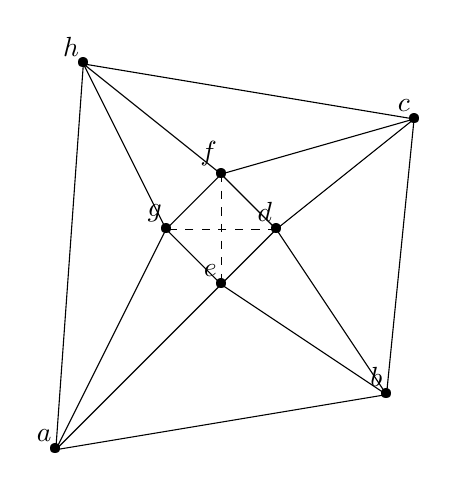
\begin{tikzpicture}[scale=0.7]
        \node[label={[label distance = -3mm]160:$a$}] at (-3, -4) {\textbullet};
        \node[label={[label distance = -3mm]160:$b$}] at (3.0, -3) {\textbullet};
        \node[label={[label distance = -3mm]160:$c$}] at (3.5, 2) {\textbullet};
        \node[label={[label distance = -3mm]160:$d$}] at (1.0, 0.0) {\textbullet};
        \node[label={[label distance = -3mm]160:$e$}] at (0, -1) {\textbullet};
        \node[label={[label distance = -3mm]160:$f$}] at (0.0, 1) {\textbullet};
        \node[label={[label distance = -3mm]160:$g$}] at (-1, 0) {\textbullet};
        \node[label={[label distance = -3mm]160:$h$}] at (-2.5, 3) {\textbullet};
        \draw (-3, -4) -- (3.0, -3);
        \draw (1.0, 0.0) -- (3.0, -3);
        \draw (3.5, 2) -- (3.0, -3);
        \draw (0, -1) -- (3.0, -3);
        \draw (1.0, 0.0) -- (3.5, 2);
        \draw (-3, -4) -- (0, -1);
        \draw (0, -1) -- (1.0, 0.0);
        \draw (-1, 0) -- (0, -1);
        \draw[dashed] (0.0, 1) -- (0, -1);
        \draw[dashed] (1, 0) -- (-1, 0);
        \draw (0.0, 1) -- (1.0, 0.0);
        \draw (0.0, 1) -- (3.5, 2);
        \draw (-3, -4) -- (-1, 0);
        \draw (-1, 0) -- (0.0, 1);
        \draw (-3, -4) -- (-2.5, 3);
        \draw (-2.5, 3) -- (-1, 0);
        \draw (-2.5, 3) -- (0.0, 1);
        \draw (-2.5, 3) -- (3.5, 2);

    \end{tikzpicture}
    \caption[Exemplo grafo de Delaunay e triangulação de Delaunay]{Para que o grafo de Delaunay
    seja uma triangulação é necessário adicionar uma das duas possíveis arestas tracejadas. O grafo
    de Delaunay da figura não é uma triangulação porque o diagrama de Voronoi desse conjunto de
    pontos tem um vértice de grau $4$.
    }\label{fig:delaunay:grafo-vs-triangulacao}
\end{figure}

Considere uma aresta $e$ de uma triangulação $T$ de $P$.
Se $e$ não faz parte do fecho convexo de $P$, então faz parte de dois triângulos adjacentes na
triangulação.
Se esses triângulos formam um quadrilátero convexo, então os vértices da aresta podem ser trocados
pelos outros dois vértices do quadrilátero, gerando uma nova triangulação.
Essa troca na aresta gera seis novos ângulos na triangulação, veja a
Figura~\ref{fig:delaunay:flip}.

\begin{figure}[H]
    \centering
    \begin{tikzpicture}
        \coordinate (a) at (-1, 0.5);
        \coordinate (b) at (4, 0);
        \coordinate (c) at (4.5, 3);
        \coordinate (d) at (0, 4);
        \draw (a) -- (b);
        \draw (b) -- (c);
        \draw (c) -- (d);
        \draw (d) -- (a);
        \draw (a) -- (c);
        \pic [draw, angle radius = 1cm] {angle = c--b--a};
        \pic [draw, angle radius = 1cm] {angle = a--c--b};
        \pic [draw, angle radius = 1cm] {angle = b--a--c};

        \pic [draw, angle radius = 0.5cm] {angle = c--a--d};
        \pic [draw, angle radius = 0.5cm] {angle = d--c--a};
        \pic [draw, angle radius = 0.5cm] {angle = a--d--c};

        \begin{scope}
            [shift={(7, 0)}]
            \coordinate (a) at (-1, 0.5);
            \coordinate (b) at (4, 0);
            \coordinate (c) at (4.5, 3);
            \coordinate (d) at (0, 4);
            \draw (a) -- (b);
            \draw (b) -- (c);
            \draw (c) -- (d);
            \draw (d) -- (a);
            \draw (b) -- (d);
            \pic [draw, angle radius = 0.5cm] {angle = c--b--d};
            \pic [draw, angle radius = 0.5cm] {angle = d--c--b};
            \pic [draw, angle radius = 0.5cm] {angle = b--d--c};

            \pic [draw, angle radius = 1cm] {angle = b--a--d};
            \pic [draw, angle radius = 1cm] {angle = d--b--a};
            \pic [draw, angle radius = 1cm] {angle = a--d--b};
        \end{scope}

    \end{tikzpicture}
    \caption[Exemplo troca de aresta]{Após trocar os vértices da aresta do quadrilátero
    convexo, seis novos ângulos se formaram.}\label{fig:delaunay:flip}
\end{figure}


Uma aresta é dita ilegal se após a troca dos vértices, o menor dos ângulos do novo quadrilátero
formado é maior que o menor dos ângulos do quadrilátero anterior a troca da aresta.
Em~\cite{computationalgeometry} é demonstrado que uma aresta $p_{i}p_{j}$ é ilegal se o ponto
$p_{l}$ do quadrilátero convexo $p_{i}p_{k}p_{j}p_{l}$ está no interior do círculo que passa por
$p_{i}p_{k}p_{j}$.
Também é demonstrado que uma triangulação que não possui arestas ilegais é uma triangulação de
Delaunay.

Isso nos dá um algoritmo para calcular a triangulação de Delaunay, podemos começar com uma
triangulação qualquer e trocar arestas que identificarmos como ilegais.
Uma possível forma de gerar uma triangulação inicial é utilizando o algoritmo de Graham, veja o
Algoritmo~\ref{alg:delaunay:delaunay-inicial}.

\begin{algorithm}[H]
    \caption[Algoritmo \textsc{delaunay} da triangulação de delaunay]{Função \textsc{delaunay}$(P)$.}
    \label{alg:delaunay:delaunay-inicial}
    \begin{algorithmic}[1]
        \Function{delaunay}{$P$}
            \State \Call{ordena}{$P$}
            \State $E \leftarrow \varnothing$
            \State \Call{adicionaAresta}{$E, P[1], P[2]$}
            \State $H[1] \leftarrow P[1]$
            \State $H[2] \leftarrow P[2]$
            \State $h \leftarrow 2$
            \For{$i \leftarrow \lk 3, \dots, |P| \rk$}
                \State \Call{adicionaAresta}{$E, P[i], P[1]$}
                \State \Call{adicionaAresta}{$E, H[h], P[i]$}
                \While{$h > 1~\AND~\Call{left}{H[h], H[h-1], P[i]}$}
                    \State $h \leftarrow h -1$
                    \State \Call{adicionaAresta}{$E, H[h], P[i]$}
                \EndWhile
                \State $h \leftarrow h + 1$
                \State $H[h] \leftarrow P[i]$
            \EndFor
            \State $\flipped \leftarrow \True$
            \While{$\flipped = \True$}
                \State $\flipped \leftarrow \False$
                \For{$e \leftarrow E$}
                    \If{\Call{illegal}{$e$}}
                        \State $\flipped \leftarrow \True$
                        \State \Call{flip}{$e$}
                    \EndIf
                \EndFor
            \EndWhile
            \State \Return $E$
        \EndFunction
    \end{algorithmic}
\end{algorithm}

As primitivas utilizadas no Algoritmo~\ref{alg:delaunay:delaunay-inicial} são os testes
\textsc{left} e \textsc{incircle}.
O teste \textsc{left} é un teste bem conhecido na geometria computacional e consiste em avaliar o
valor do seguinte determinante:
$$\textsc{left}(p_i, p_j, p_k) =
\begin{vmatrix}
    x_{p_i} & y_{p_i} & 1 \\
    x_{p_j} & y_{p_j} & 1 \\
    x_{p_k} & y_{p_k} & 1
\end{vmatrix}$$
em que um valor maior que zero significa que $p_k$ está à esquerda da reta orientada que passa por
$p_i$ e $p_j$, zero significa que $p_k$ está sobre a reta e um valor menor que zero significa que
$p_k$ está à direita da reta.

Guibas e Stolfi [\cite{guibas-stolfi}] mostram que para determinar se um ponto $p_l$ está dentro
do círculo que passa por $p_{i}p_{j}p_{k}$ podemos avaliar o valor do seguinte determinante:
$$\textsc{incircle}(p_i, p_j, p_k, p_l) =
\begin{vmatrix}
    x_{p_i} & y_{p_i} & x_{p_i}^2 + y_{p_i}^2 & 1 \\
    x_{p_j} & y_{p_j} & x_{p_j}^2 + y_{p_j}^2 & 1 \\
    x_{p_k} & y_{p_k} & x_{p_k}^2 + y_{p_k}^2 & 1 \\
    x_{p_l} & y_{p_l} & x_{p_l}^2 + y_{p_l}^2 & 1
\end{vmatrix}$$

em que um valor maior que zero significa que $p_l$ está dentro do círculo, zero significa que $p_l$
está na borda do círculo e um valor menor que zero significa que $p_l$ está fora do círculo.

Guibas, Mitchell e Roos [\cite{guibas-mitchell-roos}] propuseram uma estrutura de dados cinética
para manter a triangulação de Delaunay.
Os certificados da estrutura serão os testes de \textsc{left} e \textsc{incircle} utilizados para
assegurar que não existem arestas ilegais.
Os momentos em que ocorre uma inversão no valor desses determinantes definem o prazo de validade
destes certificados.

Um evento associado ao vencimento de um certificado do tipo \textsc{incircle} resulta na troca de
uma aresta, veja a Figura~\ref{fig:delaunay:incircle}.
Um detalhe que vale ser ressaltado é que a troca só deve ser realizada se o quadrilátero em
questão é convexo.

\begin{figure}[H]
    \centering
    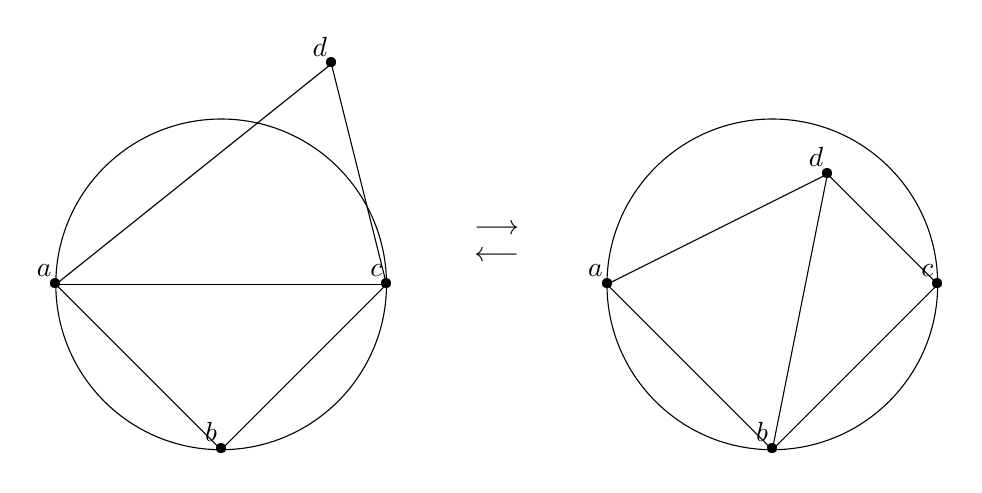
\begin{tikzpicture}[scale=0.7]
        \node[circle,draw,minimum size=4.2cm] at (0,0) {};
        \node[label={[label distance = -3mm]160:$a$}] at (-3.0, 0) {\textbullet};
        \node[label={[label distance = -3mm]160:$b$}] at (0, -3) {\textbullet};
        \node[label={[label distance = -3mm]160:$c$}] at (3, 0) {\textbullet};
        \node[label={[label distance = -3mm]160:$d$}] at (2, 4) {\textbullet};

        \draw (-3, 0) -- (0, -3);
        \draw (0, -3) -- (3, 0);
        \draw (-3, 0) -- (3, 0);
        \draw (-3, 0) -- (2, 4);
        \draw (2, 4) -- (3, 0);

        \node at (5, 1.00) {$\longrightarrow$};
        \node at (5, 0.5) {$\longleftarrow$};

        \begin{scope}
            [shift={(10, 0)}]
            \node[circle,draw,minimum size=4.2cm] at (0,0) {};
            \node[label={[label distance = -3mm]160:$a$}] at (-3.0, 0) {\textbullet};
            \node[label={[label distance = -3mm]160:$b$}] at (0, -3) {\textbullet};
            \node[label={[label distance = -3mm]160:$c$}] at (3, 0) {\textbullet};
            \node[label={[label distance = -3mm]160:$d$}] at (1, 2) {\textbullet};

            \draw (-3, 0) -- (0, -3);
            \draw (0, -3) -- (3, 0);
            \draw (1, 2) -- (0, -3);
            \draw (-3, 0) -- (1, 2);
            \draw (1, 2) -- (3, 0);
        \end{scope}

    \end{tikzpicture}
    \caption[Exemplo evento \textsc{incircle}]{Após a entrada de $d$ no círculo definido por $a$,
    $b$ e $c$, a aresta $ac$ se torna inválida e é trocada pela aresta $bd$.}
    \label{fig:delaunay:incircle}
\end{figure}

Um evento associado ao vencimento de um certificado do tipo \textsc{left} resulta na adição ou
remoção de um vértice ao fecho convexo dos pontos e na remoção ou adição de um novo triângulo na
triangulação, veja a Figura~\ref{fig:delaunay:left}.

\begin{figure}[H]
    \centering
    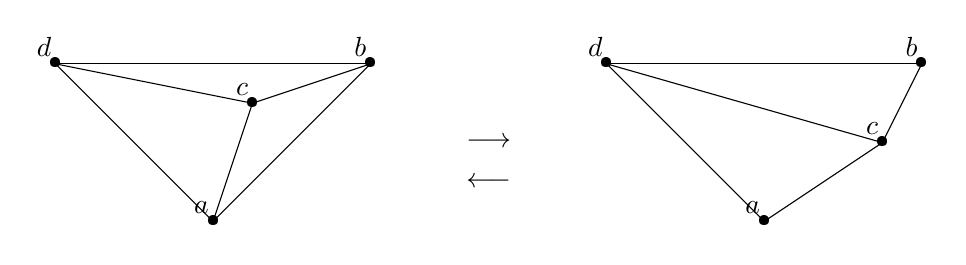
\begin{tikzpicture}
        \node[label={[label distance = -3mm]160:$a$}] at (0, 1) {\textbullet};
        \node[label={[label distance = -3mm]160:$b$}] at (2.0, 3.0) {\textbullet};
        \node[label={[label distance = -3mm]160:$c$}] at (0.5, 2.5) {\textbullet};
        \node[label={[label distance = -3mm]160:$d$}] at (-2.0, 3) {\textbullet};
        \draw (0, 1) -- (2.0, 3.0);
        \draw (0, 1) -- (0.5, 2.5);
        \draw (0.5, 2.5) -- (2.0, 3.0);
        \draw (0, 1) -- (-2.0, 3);
        \draw (-2.0, 3) -- (0.5, 2.5);
        \draw (-2.0, 3) -- (2.0, 3.0);

        \node at (3.5, 2.00) {$\longrightarrow$};
        \node at (3.5, 1.5) {$\longleftarrow$};

        \begin{scope}
            [shift={(7, 0)}]
            \node[label={[label distance = -3mm]160:$a$}] at (0, 1) {\textbullet};
            \node[label={[label distance = -3mm]160:$c$}] at (1.5, 2) {\textbullet};
            \node[label={[label distance = -3mm]160:$b$}] at (2.0, 3.0) {\textbullet};
            \node[label={[label distance = -3mm]160:$d$}] at (-2.0, 3) {\textbullet};
            \draw (0, 1) -- (1.5, 2);
            \draw (-2.0, 3) -- (1.5, 2);
            \draw (2.0, 3.0) -- (1.5, 2);
            \draw (0, 1) -- (-2.0, 3);
            \draw (-2.0, 3) -- (2.0, 3.0);
        \end{scope}
    \end{tikzpicture}
    \caption[Exemplo de evento \textsc{left}]{Exemplo de evento \textsc{left}.
    O ponto $c$ sai do fecho convexo, e por isso um triângulo é removido da triângulação.
    A Figura também pode ser vista da direita para à esquerda.}
    \label{fig:delaunay:left}
\end{figure}

Na verdade, utilizaremos uma técnica muito comum na geometria computacional para facilitar a
computação dos eventos.
Adicionaremos um ponto no infinito e uma aresta entre cada ponto no fecho convexo e esse ponto no
infinito.
Dessa forma, poderemos tratar todos eventos da mesma forma, cada evento consiste na troca de uma
aresta do quadrilátero formado pelos quatro vértices que participam do evento.
Eventos envolvendo o ponto no infinito ainda devem ter o prazo de validade
calculado através da rotina \textsc{left} com os três pontos que não são o infinito.

Além disso, em certos casos degenerados, é possível que quadriláteros adjacentes estejam
envolvidos num evento ao mesmo tempo.
Esses são os casos em que o grafo de Delaunay não corresponde à triangulação de Delaunay, com
faces que são polígonos com mais de três lados.
Isso ocorre quando mais de quatro pontos numa vizinhança se tornam co-circulares e são casos que
devem ser tratados de forma especial.
Esses casos são identificados quando os eventos da fila de prioridades ocorrem no mesmo instante,
envolvendo quadriláteros adjacentes.
A solução proposta em~\cite{aggarwal-guibas-saxe-shor} calcula uma triangulação para o
instante~$t + \epsilon$ em tempo linear, sendo $t$ o instante de ocorrência do evento.
Assim, após o processamento desses eventos a estrutura permanece correta.

A estrutura de dado cinética pode ser construída da seguinte forma:
\begin{enumerate}
    \item Calcular a triangulação de Delaunay de $P$ para os pontos na posição inicial.
    \item Para cada quadrilátero formado por triângulos adjacentes na triangulação calcular os
    prazos de validade dos certificados e inseri-los numa fila com prioridades.
    Isso inclui os quadriláteros que tem o ponto no infinito como vértice, que terão seus prazos
    de validade calculados de acordo com o zero da função \textsc{left}, e não da função
    \textsc{incircle} como os demais.
\end{enumerate}

Note que a estrutura de dados pode ser gerada independentemente do algoritmo utilizado para
calcular a triangulação de Delaunay inicial.
Isso nos permite utilizar um algoritmo mais eficiente para calcular a triangulação inicial, como o
algoritmo incremental que consome tempo $O(n\lg{n})$.
O segundo passo também consome tempo $O(n\lg{n})$, já que calcular os prazos de validade toma
tempo constante e a inserção na fila com prioridades $O(\lg{n})$.


\section{Análise de desempenho}\label{sec:delaunay:analise-de-desempenho}

As análises de desempenho aqui foram extraídas de~\cite{eduardo}.

A estrutura de dados cinética para manter a triangulação de Delaunay é uma estrutura
\textit{responsiva}, pois o custo de processar um certificado é $O(\lg{n})$.
O custo de processar um certificado é o custo de trocar uma aresta e recalcular os certificados dos
quatro quadriláteros envolvidos nessa troca.
Nos casos degenerados é mais do que quatro quadriláteros serão envolvidos, mas
em~\cite{guibas-mitchell-roos} é mostrado que o tempo amortizado continua sendo $O(\lg{n})$.

A estrutura é \textit{eficiente}, pois todos os eventos processados são eventos \textit{externos},
isto é, todo vencimento de certificado representa uma troca na descrição combinatória da
triangulação de Delaunay.
De acordo com~\cite{eduardo}, no caso de movimentos lineares, o número total de eventos é
$O(n^3)$.

A estrutura é \textit{compacta}, pois cada certificado está associado a uma aresta, teremos
$O(n)$ certificados na fila de prioridades num determinado instante.

A estrutura não é \textit{local}, pois um ponto pode estar envolvido em até $O(n)$
certificados, veja a Figura~\ref{fig:delaunay:naolocal}.

\begin{figure}[H]
    \centering
    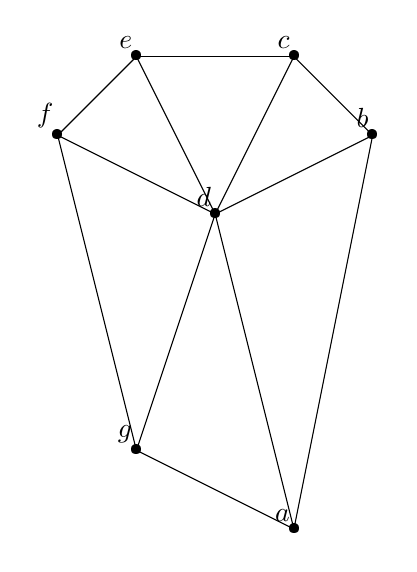
\begin{tikzpicture}
        \node[label={[label distance = -3mm]160:$a$}] at (1, -2) {\textbullet};
        \node[label={[label distance = -3mm]160:$b$}] at (2.0, 3.0) {\textbullet};
        \node[label={[label distance = -3mm]160:$c$}] at (1.0, 4) {\textbullet};
        \node[label={[label distance = -3mm]160:$d$}] at (0, 2) {\textbullet};
        \node[label={[label distance = -3mm]160:$e$}] at (-1, 4) {\textbullet};
        \node[label={[label distance = -3mm]160:$f$}] at (-2, 3) {\textbullet};
        \node[label={[label distance = -3mm]160:$g$}] at (-1, -1) {\textbullet};
        \draw (1, -2) -- (2.0, 3.0);
        \draw (0, 2) -- (2.0, 3.0);
        \draw (1.0, 4) -- (2.0, 3.0);
        \draw (1, -2) -- (0, 2);
        \draw (0, 2) -- (1.0, 4);
        \draw (-2, 3) -- (0, 2);
        \draw (-1, 4) -- (0, 2);
        \draw (-1, 4) -- (1.0, 4);
        \draw (-1, -1) -- (0, 2);
        \draw (-2, 3) -- (-1, 4);
        \draw (1, -2) -- (-1, -1);
        \draw (-1, -1) -- (-2, 3);
    \end{tikzpicture}
    \caption[Exemplo de não localidade]{Exemplo de situação em que um ponto, o ponto $d$, está
    envolvido em $O(n)$ certificados.}\label{fig:delaunay:naolocal}
\end{figure}

